\documentclass[10pt]{article}
\usepackage{multicol}   
\usepackage{graphicx}   
\usepackage{amsmath}    
\usepackage{hyperref}   
\usepackage{float}      
\usepackage{geometry}   
\usepackage{media9}
\geometry{margin=0.75in}

\usepackage[backend=bibtex,style=verbose-trad2]{biblatex}

\title{Quantum Weirdness:  Exploring Quantum Error Correction}
\author{Andry Lloyd Paez \\ San Jose State University}
\date{}

\begin{document}

\maketitle

\begin{abstract}
Quantum computers are highly susceptible to noise, which can lead to errors that jeopardize computations. Quantum Error Correction (QEC) offers a robust way to protect quantum information from such errors. This project focuses on demonstrating the efficiency of the Shor Code, one of the foundational quantum error-correcting codes. By simulating noisy quantum systems with and without error correction, we highlight the effectiveness of QEC and present results in an accessible manner for audiences new to quantum computing.
\end{abstract}

% Begin two-column layout
\begin{multicols}{2}

\section*{Introduction}
Quantum computing leverages principles like superposition and entanglement to solve problems that are infeasible for classical computers. However, noise—such as bit-flip and phase-flip errors—poses a significant challenge.

\subsection*{Motivation}
This project bridges computational physics and quantum computing to address the problem of noise in quantum systems. By visualizing and simulating the Shor Code, we aim to demonstrate how redundancy in encoding qubits mitigates errors and ensures accurate computations.

\subsection*{Goals}
The primary objectives are:
\begin{itemize}
    \item Use real quantum hardware that is susceptible to noise via IBM Channels
    \item Implement the Shor Code and redundancy code to correct errors.
    \item Compare results with and without error correction using visualizations.
\end{itemize}

\section*{Theory}
\subsection*{Basics of Quantum Computing}
A qubit can exist in a superposition state represented as:
\[
|\psi\rangle = \alpha|0\rangle + \beta|1\rangle
\]
with \( |\alpha|^2 + |\beta|^2 = 1 \).

A quantum circuit can be used to visualize these states. The qubits are represented as the wires in the diagram while the other objects represent the gates. 
\begin{figure}[H]
    \centering
    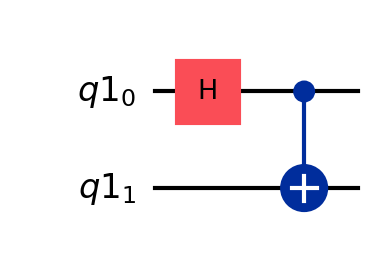
\includegraphics[width=\columnwidth]{figures/qc.png} % Placeholder
    \caption{The Bell Circuit}
    \label{fig:no_error}
\end{figure}

\begin{itemize}
    \item tensor products
    \item talk about other types of gates that I won't cover
\end{itemize}

\subsection*{Quantum Errors}
Quantum systems are prone to:
\begin{itemize}
    \item \textbf{Bit-flip errors:} \( |0\rangle \to |1\rangle \) or \( |1\rangle \to |0\rangle \).
    \item \textbf{Phase-flip errors:} Changes in the relative phase of the qubit state.
\end{itemize}

\subsection*{The Shor Code}
The Shor Code encodes one logical qubit into nine physical qubits, correcting both bit-flip and phase-flip errors through redundancy.

\section*{Methods}
\subsection*{Simulation Setup}
Simulations were performed using Qiskit to:
\begin{itemize}
    \item Generate noisy quantum circuits.
    \item Implement the Shor Code for error correction.
    \item Measure outcomes with and without error correction.
\end{itemize}

\subsection*{Tools}
We utilized:
\begin{itemize}
    \item Qiskit for quantum circuit simulation.
    \item Matplotlib for visualizations and histograms.
    \item Python for coding and animations.
\end{itemize}

\section*{Results and Discussion}
\subsection*{Noisy Circuit Without Error Correction}
\textbf{Visualization:} The histogram in Figure \ref{fig:no_error} shows a spread of results due to noise.
\begin{figure}[H]
    \centering
    % \includegraphics[width=\columnwidth]{no_error.png} % Placeholder
    \caption{Measurement results without error correction.}
    \label{fig:no_error}
\end{figure}

\subsection*{Circuit With Shor Code}
\textbf{Visualization:} The histogram in Figure \ref{fig:shor_code} demonstrates how error correction narrows the distribution to the correct outcome.
\begin{figure}[H]
    \centering
    % \includegraphics[width=\columnwidth]{shor_code.png} % Placeholder
    \caption{Measurement results with Shor Code error correction.}
    \label{fig:shor_code}
\end{figure}

\subsection*{Comparison of Results}
\textbf{Analysis:} The Shor Code improves accuracy significantly, as shown in the comparative histogram (Figure \ref{fig:comparison}).
\begin{figure}[H]
    \centering
    % \includegraphics[width=\columnwidth]{comparison.png} % Placeholder
    \caption{Comparison of results with and without error correction.}
    \label{fig:comparison}
\end{figure}

\section*{Conclusion}
This project demonstrates the critical role of quantum error correction in mitigating noise and ensuring reliable quantum computations. The Shor Code is an effective method to correct both bit-flip and phase-flip errors, making it a cornerstone for future fault-tolerant quantum computing.

\section*{Acknowledgments}
Thanks to the instructors, peers, and online resources that supported this project.

\end{multicols}

% References
\begin{thebibliography}{9}
\bibitem{bernhardt}
Chris Bernhardt, \textit{Quantum Computing for Everyone}.
\bibitem{qiskit}
Qiskit Documentation, \url{https://qiskit.org/documentation/}.
\bibitem{roffe}
Joschka Roffe, \href{http://dx.doi.org/10.1080/00107514.2019.1667078}{\textit{Quantum error correction: an introductory guide}}
\end{thebibliography}
\end{document}
